\documentclass[dvipsnames]{beamer}
\usepackage{comment}
\usepackage{hyperref}

\title{MATH 1190 \& 1210 Meeting for Week 12}
\author{Josh}
\date{23 March 2026}

\newcommand{\transition}[1]{\frame{{}\begin{center}\fbox{#1}\end{center}}}

\begin{document}

\maketitle


\section{Logistics: Pacing}

\transition{Logistics}

\frame{{Logistics: Pacing}

{\bf Where are folks in the lessons right now?}

}

\frame[t]{{Logistics: Upcoming Schedule}

    \begin{itemize}
    \item week 11 of class (23 March - 27 March)
        \begin{itemize}
        \item lesson 16 (Properties of Integration) -- {\footnotesize\color{red} last topic on assessment 3}
        \item lesson 17 (Antiderivatives \& Indefinite Integrals)
        \end{itemize}
    \item week 12 of class (30 March - 3 April)
        \begin{itemize}
        \item lesson 18 (FTOC) 
        \item lesson 19 (Summations)
        \item KC 3 on Tuesday 31 March (can change if needed)
        \item I will send the first draft of KC3 later today. Please send any comments by Wednesday 25 March so I can get it to the printers by Thursday.
        \end{itemize}
    \end{itemize}

}

\frame[t]{{Logistics: Upcoming Deadlines}

{\bf Assessment-related Logistics}
\begin{itemize}
\item The KC 2 Reflection is due on Tuesday 24 March before 11:59 PM. Good opportunity to give students feeback and promote metacognition.
\item Assessment 2 regrade requests open now until Thursday 26 March.
\item Assessment 3
    \begin{itemize}
    \item new targets: {\color{RedOrange}A2},{\color{RedOrange}A3}, {\color{Fuchsia}I1}, {\color{Fuchsia}I2}, 
    \item reassessment targets: {\color{ProcessBlue}F2}, {\color{ForestGreen}D2}, {\color{ForestGreen}D3}, {\color{RedOrange}A1}
    \item Tuesday, 31 March, 7:00 PM; 80 minutes
    \item room assignments are currently the same as KC1 unless folks feel like they won't be ready and we need to change the date.
    \end{itemize}
\end{itemize}

}




\section{Content}

\transition{Content}
\section{Next Week: Lesson Logistics (I2)}

\begin{frame}{Lesson 16 Focus (I2): Properties of Definite Integrals}
\textbf{Core Ideas:}
\begin{itemize}
\item Interpret definite integrals as \textbf{signed (net) area}
\item Compute integrals using \textbf{properties}
\end{itemize}

\vspace{0.3cm}

\textbf{Key Properties:}
\begin{itemize}
\item Break Apart Property
\item Reverse Limits Property
\item Linearity
\item Area of a Line Segment
\end{itemize}
\end{frame}

\begin{frame}{Student Learning Goals}
Students should be able to:
\begin{itemize}
\item Use geometry (triangles, rectangles, circles) to compute signed area
\item Understand when areas \textbf{cancel out}
\item Work backwards: sketch $f(x)$ from $\int_a^b f(x)\,dx$
\item Apply properties to evaluate integrals efficiently
\item We will add a formula sheet to KC3
\end{itemize}
\end{frame}

\begin{frame}{What Students Found Challenging}
\begin{itemize}
\item Signed area vs. total area
\begin{itemize}
\item Positive and negative regions canceling
\end{itemize}

\item Geometry issues:
\begin{itemize}
\item Recognizing shapes (e.g., quarter circles)
\item Finding missing dimensions (like radius)
\end{itemize}
\end{itemize}

\vspace{0.3cm}

\textbf{Takeaway:} Don’t assume geometry is automatic
\end{frame}

\begin{frame}{What Went Well}
\begin{itemize}
\item Many students found the lesson intuitive
\item Geometry connection was helpful and engaging
\item Visual reasoning supported understanding
\end{itemize}
\end{frame}



\begin{frame}{Worksheet Flow (What to Expect)}
\begin{itemize}
\item Early: interpreting signed area (triangles, basic shapes)
\item Middle:
\begin{itemize}
\item Practice with properties (Break Apart, Reverse Limits)
\end{itemize}
\item Later:
\begin{itemize}
\item Linearity + combining properties
\item Area of line segments
\end{itemize}
\item Challenge:
\begin{itemize}
\item Sketching a function from integral values
\end{itemize}
\end{itemize}
\end{frame}

\begin{frame}{Where Students Will Need Help}
\begin{itemize}
\item Moving from picture $\rightarrow$ integral
\item Moving from integral $\rightarrow$ picture
\item Combining multiple properties in one problem
\end{itemize}

\end{frame}

\begin{frame}{Core Problems to Prioritize}
\begin{itemize}
\item Example 1 / Exercise A
\item Example 2 / Exercise B
\item Exercises C, D, E, F
\end{itemize}

\vspace{0.3cm}

\textbf{If short on time:}
\begin{itemize}
\item Focus on conceptual understanding (area + properties)
\item Skip extra practice before core ideas are solid
\end{itemize}
\end{frame}

\section{Next Week: Lesson Logistics (I3)}

\begin{frame}{Lesson 17 Focus (I3): Antiderivatives}
\textbf{Core Ideas:}
\begin{itemize}
\item Antiderivative = reverse of derivative
\item Find $F(x)$ such that $F'(x) = f(x)$
\item Introduce indefinite integrals
\end{itemize}

\vspace{0.3cm}

\textbf{Connection to Previous Lesson:}
\begin{itemize}
\item Still grounded in signed area and definite integrals
\item Now shifting toward \textbf{functions}, not just numbers
\end{itemize}
\end{frame}

\begin{frame}{Student Learning Goals}
Students should be able to:
\begin{itemize}
\item Understand what an antiderivative represents
\item Use the power rule for indefinite integrals
\item Distinguish between:
\begin{itemize}
\item a \textbf{particular} antiderivative
\item a \textbf{general} antiderivative ($+C$)
\end{itemize}
\item Compute basic antiderivatives:
\begin{itemize}
\item power functions
\item exponentials
\item logarithms
\end{itemize}
\end{itemize}
\end{frame}

\begin{frame}{What Students May Struggle With}
\begin{itemize}
\item Understanding “reverse derivative” conceptually
\item Forgetting the constant of integration ($+C$)
\item Confusing definite vs. indefinite integrals
\item Memorizing rules without understanding patterns
\end{itemize}

\vspace{0.3cm}

\textbf{Big Shift:}
\begin{itemize}
\item From \textbf{numbers (area)} $\rightarrow$ \textbf{functions}
\end{itemize}
\end{frame}



\begin{frame}{Key Ideas to Highlight}
\begin{itemize}
\item Linearity of antiderivatives:
\[
\int (f(x) + g(x))\,dx = \int f(x)\,dx + \int g(x)\,dx
\]

\item Power rule:
\[
\int x^n dx = \frac{x^{n+1}}{n+1} + C \quad (n \neq -1)
\]

\item Special cases:
\begin{itemize}
\item $\int \frac{1}{x} dx = \ln |x| + C$
\item $\int e^x dx = e^x + C$
\end{itemize}
\end{itemize}
\end{frame}

\begin{frame}{Worksheet Flow (What to Expect)}
\begin{itemize}
\item Start:
\begin{itemize}
\item Definition of antiderivative
\item “What function has this derivative?”
\end{itemize}

\item Middle:
\begin{itemize}
\item Build table of common antiderivatives
\item Introduce power rule + linearity
\end{itemize}

\item Later:
\begin{itemize}
\item Combine rules
\item Practice with sums of functions
\end{itemize}
\end{itemize}
\end{frame}

\begin{frame}{Where Students Will Need Help}
\begin{itemize}
\item Recognizing patterns (reverse derivative thinking)
\item Applying linearity correctly
\item Remembering and interpreting $+C$
\item Transitioning from examples to general rules
\end{itemize}
\end{frame}

\begin{frame}{Core Problems to Prioritize}
\begin{itemize}
\item Example 1 / Exercise A
\item Example 2 / Exercise B
\item Exercises C
\end{itemize}

\vspace{0.3cm}

\textbf{If short on time:}
\begin{itemize}
\item Focus on understanding antiderivatives conceptually
\item Prioritize power rule + linearity
\end{itemize}
\end{frame}


\section{Pedagogy}

\transition{Pedagogy}


\transition{Active Learning}
\transition{And Now - An Active Learning Discussion with Josh!}



% Slide 1
\begin{frame}{Active Learning Activity: Red Light, Green Light}
\begin{itemize}
    \item Students work in groups of 3--4
    \item Each group works on similar problems using small whiteboards or wall boards
    \item Each group receives:
    \begin{itemize}
        \item A green marker (for understood ideas)
        \item A red marker (for unclear ideas)
    \end{itemize}
    \item Students write:
    \begin{itemize}
        \item \textcolor{green}{Green: What they understand}
        \item \textcolor{red}{Red: What they do not understand}
    \end{itemize}
\end{itemize}
\end{frame}

% Slide 2
\begin{frame}{Class Implementation}
\begin{itemize}
    \item 36 students divided into 9 groups (1--9)
    \item Each group received problems A, B, and C
    \item Problem assignment based on group number:
    \begin{itemize}
        \item Groups divisible by 3: Problem A (3, 6, 9)
        \item Remainder 1: Problem B (1, 4, 7)
        \item Remainder 2: Problem C (2, 5, 8)
    \end{itemize}
    \item After 20 minutes, groups rotated:
    \begin{itemize}
        \item A $\rightarrow$ B $\rightarrow$ C $\rightarrow$ A
    \end{itemize}
    \item Each group attempted all problems
\end{itemize}
\end{frame}
\begin{frame}
\centering
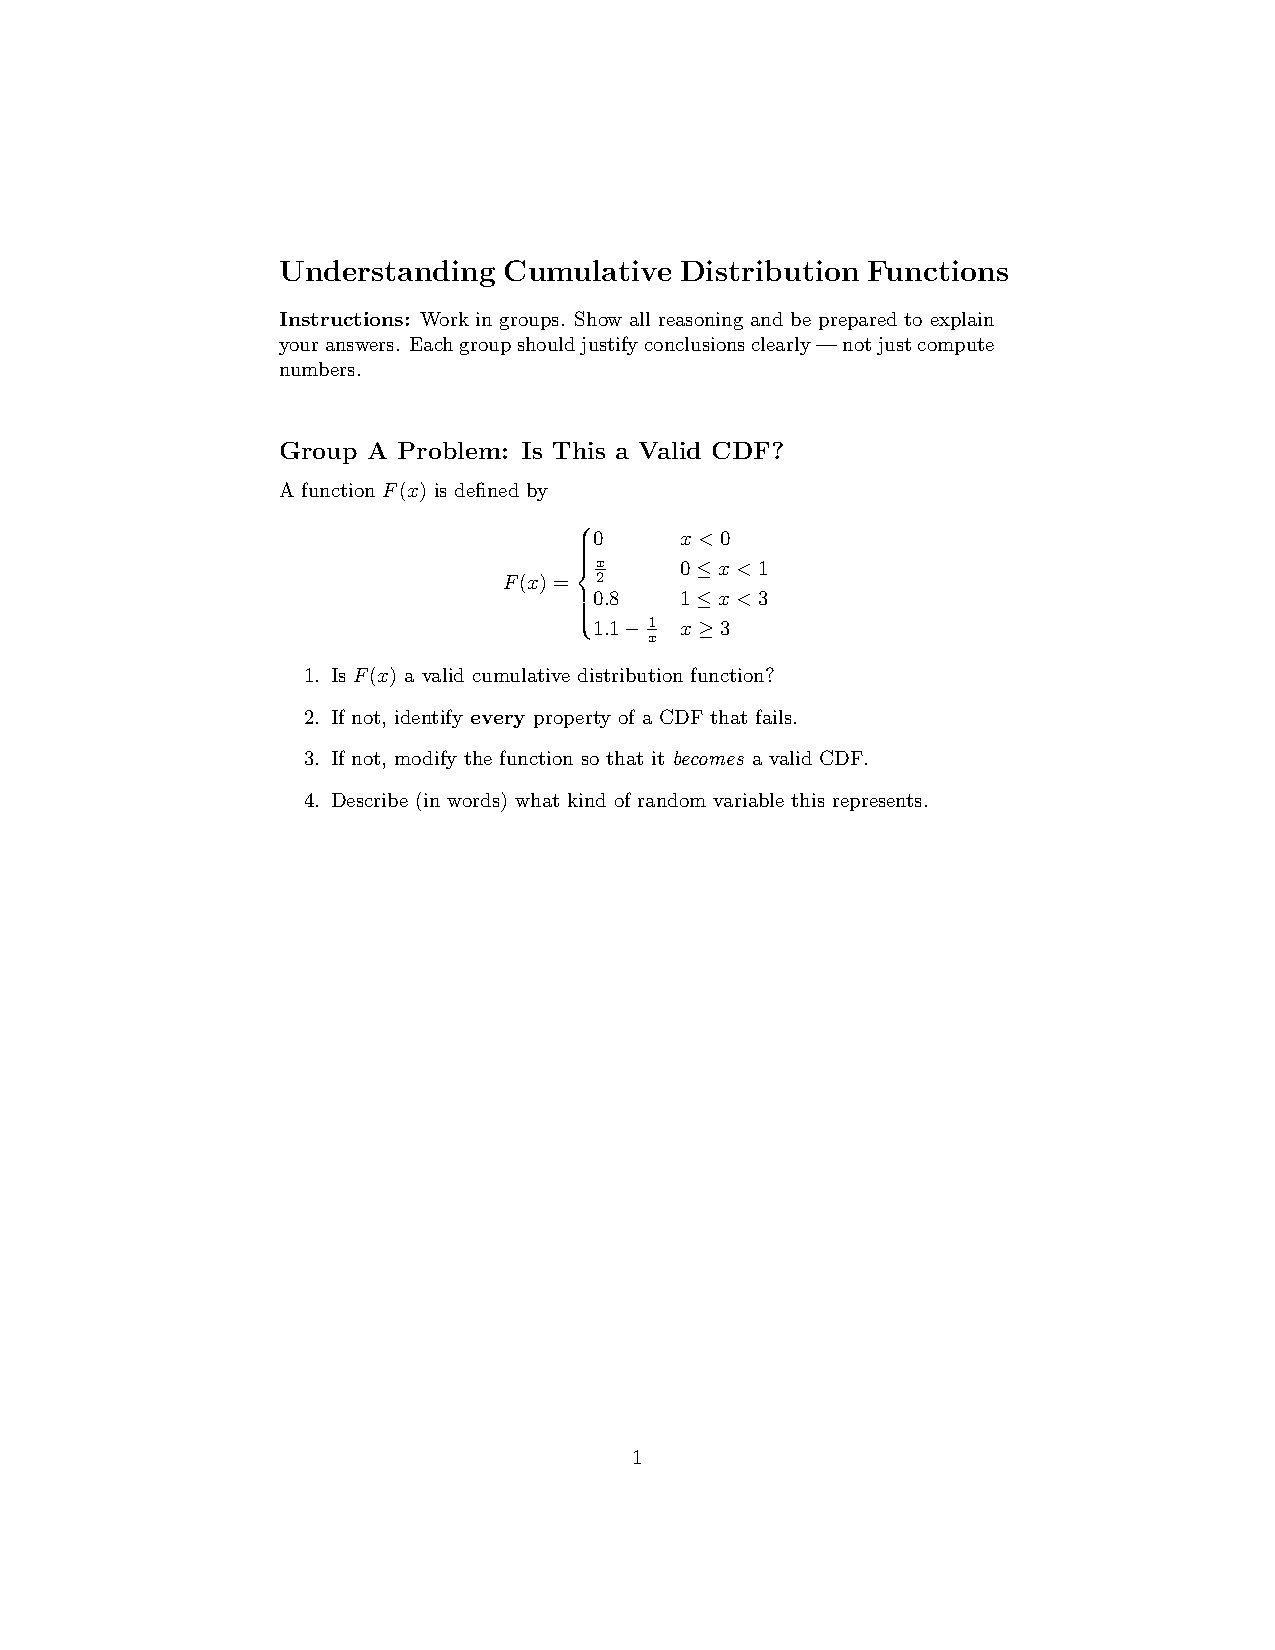
\includegraphics[width=\textwidth,page=1]{CDFActiveLearning.pdf}
\end{frame}
\begin{frame}
\centering
\includegraphics[width=\textwidth,page=2]{CDFActiveLearning.pdf}
\end{frame}
\begin{frame}
\centering
\includegraphics[width=\textwidth,page=3]{CDFActiveLearning.pdf}
\end{frame}
% Slide 3
\begin{frame}{Results: Pros}
\begin{itemize}
    \item Red responses promoted discussion during instructor walkthroughs
    \item Provided insight into student understanding
    \item Encouraged metacognition
    \item Increased student ownership of learning
\end{itemize}
\end{frame}

% Slide 4
\begin{frame}{Results: Cons}
\begin{itemize}
    \item Some students did not write anything in red
    \item Students were sometimes reluctant to use whiteboards
    \item Occasional dominance by one group member
    \item Problem assignment method was overly complex and time-consuming
\end{itemize}
\end{frame}

% Slide 5
\begin{frame}{Conclusion}
\begin{itemize}
    \item Would use this activity again
    \item Likely more effective with smaller groups
    \item Easier to implement in active learning classrooms
    \item Additional support (e.g., learning assistants, more boards) would help
\end{itemize}
\end{frame}

%%%%%%%%%%%%%%%%%%%%%%%%%%%%%%%%%%%%%%%%%%%%%%%%%%%%%%%%%%%%%%%%%%%%%%%%%%%%%%%%%%%%%%%%%%%%%%%%%%%%%%%%%%%%%%%%%%%%%%%%%%%%%%%%%%%%%%%%%%%%%%%%%%%%%%%%%%%%%%%%%%%%%%%%%%%%%%%%%%%%%%%%%%%%%%%%%%%%%%%%%%%%%%%%%%%%%%%%%%%%%%%%%%%%%%%%%%%%%%%%%%%%%%%%%%%%%%%%%%%%%%%%%%%%%%%%%%%%%%%%%%%%
\section{Pedagogy}

\transition{Commom Classroom Scenarios}


\begin{frame}{Scenario 1: “Just Show Me How”}
\textbf{Situation:}
When walking around to answer questions from students, a student (or group) says:
\begin{quote}
“Can you just show us how to do this one? I have no idea even where to start.”
\end{quote}
\begin{itemize}
    \item What things have you noticed that work?
    \item What doesn’t work?
    \item What strategies feel natural?
    \item How can the concept of \emph{productive struggle} influence how we design group tasks?
\end{itemize}
\end{frame}
\begin{comment}
They are working on:
\[
\frac{d}{dx}(x^2 e^x)
\]

\vspace{0.3cm}

\textbf{Task:}
\begin{itemize}
\item One person plays the LA
\item One person plays the student
\item Act out the interaction (1--2 minutes)
\end{itemize}

\vspace{0.3cm}

\textbf{Goal:}
\begin{itemize}
\item Help without taking over
\item Encourage student thinking
\end{itemize}
\end{comment}
%%%%%%%%%%%%%%%%%%%%%%%%%%%%%%%%%%%%%%%%%%%%%%%%%%%%%%%%%%%%%%%%%%%%%%%%%%%%%%%%%%%%%%%%%%%%%%%%%%%%%%%%%%%%%%%%%%%%%%%%%%%%%%%%%%%%%%%%%%%%%%%%%%%%%%%%%%%%%%%%%%%%%%%%%%%%%%%%%%%%%%%%%%%%%%%%%%%%%%%%%%%%%%%%%%%%%%%%%%%%%%%%%%%%%%%%%%%%%%%%%%%%%%%%%%%%%%%%%%%%%%%%%%%%%%%%%%%%%%%%%%%%
\begin{frame}{Scenario 2: Silence in the Classroom}
\textbf{Situation:}

You ask:
\begin{quote}
“What does the derivative represent here?”
\end{quote}

No one responds. The room is completely silent.
\begin{itemize}
    \item What things have you noticed that work?
    \item What doesn’t work?
    \item What strategies feel natural?
\end{itemize}
\end{frame}

\begin{comment}
\vspace{0.3cm}

\textbf{Task:}
\begin{itemize}
\item Act out how you respond in real time
\item What do you say next?
\item What do you \emph{not} do?
\end{itemize}

\vspace{0.3cm}

\textbf{Goal:}
\begin{itemize}
\item Get students talking
\item Reduce pressure
\item Avoid answering your own question immediately
\end{itemize}
\end{comment}
%%%%%%%%%%%%%%%%%%%%%%%%%%%%%%%%%%%%%%%%%%%%%%%%%%%%%%%%%%%%%%%%%%%%%%%%%%%%%%%%%%%%%%%%%%%%%%%%%%%%%%%%%%%%%%%%%%%%%%%%%%%%%%%%%%%%%%%%%%%%%%%%%%%%%%%%%%%%%%%%%%%%%%%%%%%%%%%%%%%%%%%%%%%%%%%%%%%%%%%%%%%%%%%%%%%%%%%%%%%%%%%%%%%%%%%%%%%%%%%%%%%%%%%%%%%%%%%%%%%%%%%%%%%%%%%%%%%%%%%%%%%%
\begin{frame}{Scenario 3: Dominating Student}
\textbf{Situation:}

One student:
\begin{itemize}
\item answers every question
\item speaks confidently
\item interrupts others
\end{itemize}

Other students are disengaged.
\begin{itemize}
    \item What things have you noticed that work?
    \item What doesn’t work?
    \item What strategies feel natural?
    \item Considering students with different confidence levels. How can we design interventions that \emph{empower quieter students without discouraging more vocal ones}?
\end{itemize}
\end{frame}

\begin{comment}
\vspace{0.3cm}

\textbf{Task:}
\begin{itemize}
\item Act out how you handle this situation
\item Keep the strong student engaged
\item Bring others into the conversation
\end{itemize}

\vspace{0.3cm}

\textbf{Goal:}
\begin{itemize}
\item Balance participation
\item Create an inclusive environment
\end{itemize}
\end{comment}


%%%%%%%%%%%%%%%%%%%%%%%%%%%%%%%%%%%%%%%%%%%%%%%%%%%%%%%%%%%%%%%%%%%%%%%%%%%%%%%%%%%%%%%%%%%%%%%%%%%%%%%%%%%%%%%%%%%%%%%%%%%%%%%%%%%%%%%%%%%%%%%%%%%%%%%%%%%%%%%%%%%%%%%%%%%%%%%%%%%%%%%%%%%%%%%%%%%%%%%%%%%%%%%%%%%%%%%%%%%%%%%%%%%%%%%%%%%%%%%%%%%%%%%%%%%%%%%%%%%%%%%%%%%%%%%%%%%%%%%%%%%%
% Slide 4
\begin{frame}{Scenario 4: Students Not Going to the Board}
\textbf{Scenario:} Some students hesitate to go to the board due to anxiety or shyness.  
\begin{itemize}
    \item What things have you noticed that work?
    \item What doesn’t work?
    \item What strategies feel natural?
    \item What kinds of activities could we implement that might help students that have high levels of social anxiety feel comfortable to contribute?
\end{itemize}
\end{frame}

\begin{comment}

\textbf{Solutions:}
\begin{itemize}
    \item Use random selection (e.g., cards, apps) to ensure equal participation.
    \item Encourage group or pair work before presenting to reduce pressure.
    \item Praise effort and participation, not just correctness.
    \item Provide alternative ways to participate (desk whiteboards, digital boards).
\end{itemize}
\end{comment}
%%%%%%%%%%%%%%%%%%%%%%%%%%%%%%%%%%%%%%%%%%%%%%%%%%%%%%%%%%%%%%%%%%%%%%%%%%%%%%%%%%%%%%%%%%%%%%%%%%%%%%%%%%%%%%%%%%%%%%%%%%%%%%%%%%%%%%%%%%%%%%%%%%%%%%%%%%%%%%%%%%%%%%%%%%%%%%%%%%%%%%%%%%%%%%%%%%%%%%%%%%%%%%%%%%%%%%%%%%%%%%%%%%%%%%%%%%%%%%%%%%%%%%%%%%%%%%%%%%%%%%%%%%%%%%%%%%%%%%%%%%%%
% Slide 5
\begin{frame}{Scenario 5: Disengaged Students}
\textbf{Scenario:} Some students appear bored or distracted during lessons often playing on phones or doing other things on laptops.  
\begin{itemize}
    \item What things have you noticed that work?
    \item What doesn’t work?
    \item What strategies feel natural?
    \item How can we ensure that our students are actually being active in their learning process?
\end{itemize}
\end{frame}

\begin{comment}
\textbf{Solutions:}
\begin{itemize}
    \item Incorporate active learning: discussions, polls, hands-on activities.
    \item Connect material to real-life examples relevant to students.
    \item Offer choices in assignments or topics to increase engagement.
    \item Break lessons into shorter segments with interactive moments.
\end{itemize}
\end{comment}
%%%%%%%%%%%%%%%%%%%%%%%%%%%%%%%%%%%%%%%%%%%%%%%%%%%%%%%%%%%%%%%%%%%%%%%%%%%%%%%%%%%%%%%%%%%%%%%%%%%%%%%%%%%%%%%%%%%%%%%%%%%%%%%%%%%%%%%%%%%%%%%%%%%%%%%%%%%%%%%%%%%%%%%%%%%%%%%%%%%%%%%%%%%%%%%%%%%%%%%%%%%%%%%%%%%%%%%%%%%%%%%%%%%%%%%%%%%%%%%%%%%%%%%%%%%%%%%%%%%%%%%%%%%%%%%%%%%%%%%%%%%%
% Slide 6
\begin{frame}{Scenario 6: Promoting Inclusivity}
\textbf{Scenario:} Students have diverse abilities, backgrounds, and learning styles. Many may struggle with material or explanations that we give in the classroom while others may feel the material is too easy. How do you approach instruction to make students feel included and confident enough to add to group discussions?
\begin{itemize}
    \item What things have you noticed that work?
    \item What doesn’t work?
    \item What strategies feel natural?
    \item What kinds of activities could we implement that might create an atmosphere of inclusivity where no one feels left out?
\end{itemize}
\end{frame}

\begin{comment}
\textbf{Solutions:}
\begin{itemize}
    \item Use differentiated instruction tailored to varying skill levels.
    \item Encourage collaborative learning and peer mentoring.
    \item Include diverse perspectives and culturally relevant materials.
    \item Allow multiple ways for students to participate (verbal, written, digital).
\end{itemize}
\end{comment}
%%%%%%%%%%%%%%%%%%%%%%%%%%%%%%%%%%%%%%%%%%%%%%%%%%%%%%%%%%%%%%%%%%%%%%%%%%%%%%%%%%%%%%%%%%%%%%%%%%%%%%%%%%%%%%%%%%%%%%%%%%%%%%%%%%%%%%%%%%%%%%%%%%%%%%%%%%%%%%%%%%%%%%%%%%%%%%%%%%%%%%%%%%%%%%%%%%%%%%%%%%%%%%%%%%%%%%%%%%%%%%%%%%%%%%%%%%%%%%%%%%%%%%%%%%%%%%%%%%%%%%%%%%%%%%%%%%%%%%%%%%%%
% Slide 7
\begin{frame}{Scenario 7: Promoting Ownership}
\textbf{Scenario:} Students are passive learners and disengaged from their own learning. How do you approach the problem of giving students more ownership of not only the classroom, but also of their own learning?
\begin{itemize}
    \item What things have you noticed that work?
    \item What doesn’t work?
    \item What strategies feel natural?
    \item In what ways could we structure our teaching to encourage students to become \emph{self-directed learners}, not just responders?
\end{itemize}
\end{frame}

\begin{comment}
\textbf{Solutions:}
\begin{itemize}
    \item Provide choices in projects and methods of learning.
    \item Encourage goal-setting and self-assessment.
    \item Incorporate project-based learning with student-led decisions.
    \item Recognize effort and initiative, not just grades.
\end{itemize}
\end{comment}




\begin{frame}{More Discussion Questions}
\begin{enumerate}
    \item What strategies could we implement to foster a classroom culture where students \emph{question and critique each other’s reasoning respectfully}?
    \item How might our feedback practices encourage students to \emph{reflect on their problem-solving process} instead of only focusing on final answers?
    \item What small, consistent teaching habits could help us build \emph{trust and approachability} over a semester?
\end{enumerate}
\end{frame}
\end{document}











\section{Big Ideas from the MAA Handbook}

\begin{frame}{Big Ideas from the Handbook}
\begin{itemize}
\item Good teaching is simple, but intentional
\item Students learn by doing, not watching
\item Recitation is not a second lecture
\item Clear expectations matter
\end{itemize}
\end{frame}

\begin{frame}{Good Teaching = Simple Habits}
\begin{itemize}
\item Speak clearly and write legibly
\item Be organized and prepared
\item Explain ideas step by step
\item Be approachable and respectful
\end{itemize}
\end{frame}

\begin{frame}{The Syllabus is a Contract}
\begin{itemize}
\item Sets expectations for everyone
\item Defines grading and policies
\item Consistency builds trust
\item Avoid changing rules mid-semester
\end{itemize}
\end{frame}

\begin{frame}{Study Sessions are Not Lectures}
\begin{itemize}
\item Avoid re-teaching lectures
\item Focus on student thinking
\item Use problems as the main tool
\item Let students do the work
\end{itemize}
\end{frame}

\begin{frame}{Students Learn by Doing}
\begin{itemize}
\item Active participation is essential
\item Group work and discussion help
\item Struggle is part of learning
\item Your role: guide, not tell
\end{itemize}
\end{frame}

\begin{frame}{Grading Should Reflect Thinking}
\begin{itemize}
\item Reward reasoning, not just answers
\item Give partial credit for good work
\item Look for understanding in steps
\item Be consistent and transparent
\end{itemize}
\end{frame}

\begin{frame}{Motivation Matters}
\begin{itemize}
\item Students ask: “Why does this matter?”
\item Connect ideas to applications
\item Show enthusiasm for the material
\item Make math feel meaningful
\end{itemize}
\end{frame}

\begin{frame}{Levels of Understanding}
\begin{itemize}
\item Recall: definitions, formulas
\item Understand: explain ideas
\item Apply: solve problems
\item Analyze/Evaluate: deeper thinking
\end{itemize}
\end{frame}

\begin{frame}{Common Teaching Pitfalls}
\begin{itemize}
\item Talking too much
\item Giving answers too quickly
\item Dismissing student questions
\item Treating teaching as secondary
\end{itemize}
\end{frame}

\begin{frame}{Key Takeaway}
\begin{itemize}
\item Teaching is not telling
\item Learning requires effort from students
\item Your goal: create opportunities to think
\end{itemize}
\end{frame}


\begin{frame}{Your Role as an LA}
\begin{itemize}
\item Not a mini-professor
\item Not just a grader
\item You are a facilitator of student thinking
\item Help students engage with calculus actively
\end{itemize}
\end{frame}

\begin{frame}{What Students Struggle With}
\begin{itemize}
\item Concept vs. computation
\item Interpreting derivatives and integrals
\item Translating word problems into math
\item Knowing \emph{why} methods work
\end{itemize}
\end{frame}

\begin{frame}{Productive Struggle}
\begin{itemize}
\item Learning happens when students think
\item Don’t remove difficulty too quickly
\item Give hints, not solutions
\end{itemize}
\end{frame}

\begin{frame}{Bad vs Good Teaching Behavior}
\textbf{Bad:}
\begin{itemize}
\item Solving the problem on the board
\item Talking most of the time
\item Giving answers too quickly
\end{itemize}

\vspace{0.3cm}

\textbf{Good:}
\begin{itemize}
\item Asking guiding questions
\item Letting students struggle productively
\item Encouraging group discussion
\end{itemize}
\end{frame}

\begin{frame}{Example: Derivative Question}
Instead of:
\[
\frac{d}{dx}(x^2 \sin x)
\]

Ask:
\begin{itemize}
\item What rules might apply here?
\item What are the two functions?
\item What happens if we treat this as a product?
\end{itemize}
\end{frame}


\begin{frame}{Common UVA Student Behaviors}
\begin{itemize}
\item “Just show me how to do it”
\item Focus on exams over understanding
\item Hesitant to speak in groups
\end{itemize}

\textbf{Your response:}
\begin{itemize}
\item Redirect with questions
\item Normalize confusion
\item Build participation gradually
\end{itemize}
\end{frame}
\section{LA Scenarios}

\end{document}

%%%%%%%%%%%%%%%%%%%%%%%%%%%%%

\frame[t]{{Pedagogy}

The article frames that the snowball effect as a challenge made more prominent by alternative grading systems, but not a bug: 

\

``I think this experience, where you have to move on to concept N+1 before you have fully mastered concept N, is normal in our own experiences as learners. Sometimes we can’t fully grasp a concept or topic until we move on to something higher, requiring us to put that earlier concept on the back burner for a while...The lesson here is that while the “snowball effect” might be inevitable in situations where you get more than one opportunity to demonstrate learning, and while it might be ideal for you while it happens, it’s not a critical flaw in alternative grading – it’s just a normal part of the nonlinear nature of learning things."

\

Traditional methods almost by definition do not have this snowball effect (unless you count studying for a final exam). But this is because they don’t have feedback loops. By removing the loop, you remove the snowballing. That is a partial win for students, because they never have to deal with shoring up skill on old topics while new ones are emerging; but it’s also a big loss, for the same reason. On balance, students are better off having feedback loops with the possibility of a snowball than they are without feedback loops and no snowball."

}
